%%%%%%%%%%%%%%%%%%%%%%%%%%%%%%%%%%%%%%%%%%%%%%%%%%%%%%%%%%%%%%%%%%%%
%           Auteur :  P.TRAN BA, E.BOUTTIER, J.SHI, E.ABIA         %
%         Création :  18/01/2012 17:05                             %
%%%%%%%%%%%%%%%%%%%%%%%%%%%%%%%%%%%%%%%%%%%%%%%%%%%%%%%%%%%%%%%%%%%%

\documentclass[a4paper,11pt]{article}

%\usepackage[utf8]{inputenc}
%\usepackage[T1]{fontenc}
%\usepackage{xunicode}
\usepackage{fontspec}
\defaultfontfeatures{Mapping=tex-text,Scale=MatchLowercase}
\usepackage{a4wide}
\usepackage{verbatim}
\usepackage{polyglossia}
\setdefaultlanguage{french}
%~ \usepackage{listings}
%\usepackage[french]{babel}
%~ \usepackage{url}
%~ \usepackage{times}
\usepackage{minted}
\usepackage{amssymb}
\usepackage{graphicx}
% graphviz.tex
% originally written by Derek Rayside, November 2003
% following an idea that Daniel Jackson implemented in his Tagger program
%
% parameters to \digraph:
% 1 - parameters for \includegraphics (optional; default value is "scale=1")
% 2 - name of the digraph
% 3 - body of the digraph

\newcommand{\digraph}[3][scale=1]{
    \newwrite\dotfile
    \immediate\openout\dotfile=#2.dot
    \immediate\write\dotfile{digraph #2 {\string#3}}
    \immediate\closeout\dotfile
    \IfFileExists{#2.ps}
        % the postscript exists: include it
        { \includegraphics[#1]{#2} }
        % the postscript doesn't exist: tell the user how to create it
        { \fbox{ \begin{tabular}{l}
            The file \texttt{#2.ps} hasn't been created from
            \texttt{#2.dot} yet. \\
            Run `\texttt{dot -Tps -o #2.ps #2.dot}' to create it. \\
            Here is a \textsf{bash} loop to process all \textsf{dot} files
            in the current directory: \\
            \texttt{
            for f in *.dot do ; 
            dot -Tps -o \$\{f\%dot\}ps \$f ; 
            done
            }
            \end{tabular}}
        }
}



\usepackage{geometry}
\geometry{hmargin=2.5cm,vmargin=1.5cm}

\title{Projet C\\Simulation d'un commutateur de niveau 3\\Rapport}
\author{Philippe \textsc{Tran Ba}, Élie \textsc{Bouttier}, Jiajun \textsc{Shi}, Émilie \textsc{Abia}\\Groupe 15}
\date\today

\begin{document}

\maketitle

\begin{abstract}

Ce rapport porte sur un projet de programmation d'un commutateur de niveau 3 en langage C. Il y est abordé le fonctionnement global du programme, suivi des choix techniques effectués afin de palier aux problèmes rencontrés. Il termine par une conclusion sur l'état du projet et des améliorations qui pourraient y être apportées.

\end{abstract}

\tableofcontents

\newpage

\section{Introduction}
\subsection{Préface}

Dans le cadre de notre préparation au diplôme d'ingénieur en Télécommunications et Réseaux, nous avons été amenés à effectuer notre projet de première année sous l'encadrement de Jérôme Ermont. Le but de ce projet était surtout de nous faire manipuler le langage C et la gestion de la mémoire mais il nous a également permis de modéliser une solution réseau simple.

La commutation de paquets, technique utilisée dans le transfert de données dans les réseaux informatiques, permet de rediriger les packets sur un lien physique particulier suivant des critères précis, avec éventuellement une modification de ceux-ci. Au vue de notre formation, le choix de la réalisation d'un simulateur de commutateur se trouve être pertinent et intéressant.

Ce rapport est composé de deux parties. La première partie présente l'application dans sa globalité, son fonctionnement. La seconde partie est consacrée au détail de l'implémentation. Enfin nous conclurons sur les apports personnels obtenus à la fin de ce projet.

\subsection{Rappel du sujet}

Nous avons effectué notre projet langage C de première année sous l'encadrement de Jérôme Ermont. Il était question principalement de simuler le fonctionnement d'un commutateur de niveau 3. 

Ainsi il s'agissait dans ce projet de simuler le travail d'un élément réseau dont le rôle serait de recevoir des trames, de les assembler pour reformer des paquets et d'effectuer par la suite la commutation de ces paquets. Les paquets routés sont à nouveau fragmentés et les trames obtenues sont stockées dans des queues selon leur priorité.

La première étape a été l'étude préalable de l'élément réseau impliqué, il s'agissait d'assimiler les fonctionnalités attendues de celui-ci et de, relativement à notre compréhension du sujet, réfléchir à un algorithme.

Dans un second temps, après nous être mis d'accord sur le modèle retenu nous nous sommes départagé le travail afin de gagner du temps.  

Nous avons ensuite regroupé notre travail et avons modifié la structure générale afin de l'optimiser au maximum. 

Enfin, il faut remarquer que notre application est vouée à évoluer : il serait par exemple souhaitable que le commutateur soit capable de mieux traiter les erreur (reprise sur erreur, renvoie...)

\section{Implémentation}
\subsection{Architecture globale de l'application}

Notre application ayant attrait au réseau, il est naturel de la décomposer en module indépendant à l'image des couches du modèle OSI. De plus, une telle décomposition rend notre solution évolutive. Il sera aisé de remplacer un module ou d'en ajouter. Sa décomposition en module assure aussi sa stabilité.

Le simulateur est lancé par la méthode \texttt{simulate} du module \texttt{simulator}. Les paramètres de lancement sont obtenue par le module \texttt{main}, en charge d'analyser les arguments de la ligne de commande. La simulation est commandé par le fichier d'entrée, comportant des instructions \texttt{IN} et des instruction \texttt{out}, dictant l'entrée ou la sortie d'un packet.

Lors de la lecture d'une instruction \texttt{IN}, le module \texttt{trame} sera appelé afin de lire une trame depuis le fichier d'entrée. Celle-ci est alors rangée dans une structure de données nommé \texttt{ListPacketFrag}, en attandant d'obtenir toute les trames d'un même paquet. C'est donc une liste chaîné, contenant dans chaque cellule un \texttt{PacketFrag} – paquet fragmenté – contenant un tableau de trame, remplit au fur et à mesure de leur arrivée. Lorsque toute les trames d'un même paquet sons reçu, le paquet fragmenté est retiré de la liste \texttt{ListPacketFrag}, afin d'être envoyé au module \texttt{packet}, en charge de l'assemblage. Le schéma ci-après résume le stockage des données dans les différentes structures.

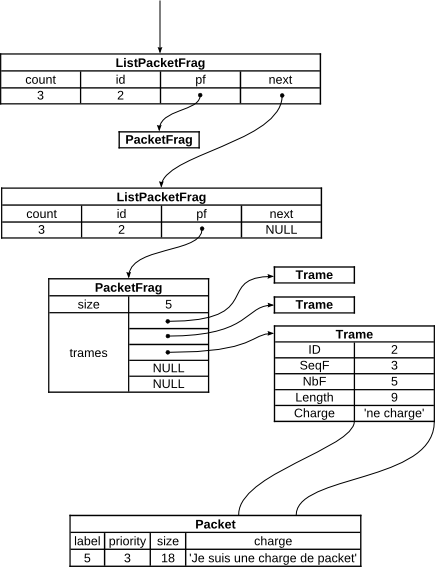
\includegraphics{s1.png}

Un paquet étant reconstitué, celui-ci est envoyé au module \texttt{commut}, en charge de sa commutation. Celui-ci modifie son label en concordance avec la table de commutation, et indique au simulateur le lien de sortie. Celui-ci va alors demander au module \texttt{packet} de le fragmenter, avant de l'envoyer dans la \texttt{queue} dédié au lien de sortie précédement établit.

Lors d'une instruction \texttt{OUT}, le module \texttt{queue} est appelé afin d'envoyer une trame sur le lien de sortie concernée et donc de l'écrire dans un fichier de sortie. La trame sortie est sélectionnée selon sa priorité de manière circulaire sauf la priorité absolue, qui elle, est envoyée immédiatement après un \texttt{OUT}.

\subsection{Détail des modules}

\subsubsection{trame}
Le module \texttt{trame} propose une fonction de décodage dont le prototype est le suivant :
\begin{minted}{c}

\end{minted}
\begin{minted}[linenos,tabsize=4]{c}
typedef struct {
  unsigned short int id; /* numéro du paquet */
  unsigned short int seqf; /* numéro de séquence */
  unsigned short int nbf; /* nombre de séquence */
  unsigned int length; /* longeur de charge */
  unsigned char * charge; /* contenue */
} Trame;
\end{minted}
Le décodage se fait en telles étapes :
\begin{enumerate}
 \item initialiser une variable de crc afin d'effectuer le contrôle d'erreur
 \item abandonner toutes les informations redondantes avant que l'on rencontre un fanion afin d'assurer le départ du décodage.
 \item Pour chaque octet utile reçu, faire l'opération \textit{ou exclusif} avec l'ancien crc pour générer le nouveau crc.
 \item Pour transformer les octets en attributs d'une trame, on décale le premier octet à gauche de 8 bits et l'opération \textit{ou} avec le deuxième octet afin de construire les attributs de 16 bits.
 \item Lors que l'on rencontre un banaliseur, on récupère l'octet suivant.
 \item Lors que l'on rencontre un fanion, la lecture de la séquence de bits est terminée et on récupère le dernier élément dans partie de charges comme le crc original.
 \item Refaire l'opération \textit{ou exclusif} entre crc calculé et le crc original, afin d'obtenir un crc pour la trame sauf les fanion et le crc original.
 \item Faire la comparaison entre le crc calculé et le crc original, s'ils sont identiques, la trame est reçue correctement, sinon, on ignore cette trame et elle est détruite.
\end{enumerate}
\subsubsection{packetfrag}
\texttt{packetfrag} correspond à un module gérant les fragments de paquets, ou les trames d'un même paquet. Un packetfrag contient, comme ci dessous, une trame ainsi que la taille du paquet auquel elle appartient :\begin{minted}{c}
struct PacketFrag {
    // Nombre de fragment (taille du tableau)
    int size;
    // Tableau contenant les trames
       Trame ** trames;
};
typedef struct PacketFrag PacketFrag;
\end{minted}
\subsubsection{listpacketfrag}
\texttt{listepacketfrag} est un module qui définit la structure des maillons de la liste chainé qui contient les fragments de paquet. 
\begin{minted}[linenos,tabsize=4]{c}
 struct ListPacketFrag {
    // Nombre de trame stocké dans le packet fragmenté
    int count;
    // ID du packet associé
    int id;
    // Packet fragmenté de la cellule
    PacketFrag * pf;
    // Cellule suivante
    struct ListPacketFrag * next;
};
typedef struct ListPacketFrag ListPacketFrag;
\end{minted}
\texttt{listepacketfrag} contient l'ID du paquet associé afin de savoir si une trame appartient au paquet concerné ou non. Elle contient aussi un compteur qui permet de savoir si le paquet est complet dans la mesure où toutes les trames attendues sont arrivées.
\subsubsection{packet}
\texttt{Packet} est un module contenant la structure qui représentera à nos yeux une trame définie comme ci dessous:
\begin{minted}[linenos,tabsize=4]{c}
 struct Packet {
  unsigned int label;
  unsigned char priority;
  unsigned int size;
  unsigned char * charge;
};

typedef struct Packet Packet;
\end{minted}
Ce modules est aussi chargé de l'assemblage et de la re-fragmentation du paquet en de multiple trames via les deux fonctions qui suivent :
\begin{minted}[linenos,tabsize=4]{c}
/* Assembler un packet */
void packet_assemble(Packet * packet, PacketFrag * pf);

/* Fragmenter un packet */
void packet_split(PacketFrag ** pf, Packet * packet, int outputsize);
\end{minted}
\subsubsection{commut}

\subsubsection{queue}
\texttt{Queue} est un module gérant les files d'attente ainsi que les 256 priorités. Une queue est une structure comportant un pointeur vers une autre queue comme ci dessous :
\begin{minted}{c}
 struct Queue {
    struct Queue * previous;
    Trame * element;
};
typedef struct Queue Queue;
\end{minted}
Chaque queue sera attribuée à une priorité et contiendra une liste chaînée de Trame. Les 256 queues des 256 priorités sont stockées dans un tableau de 256 queue dont l'indice représente la priorité. Zéro étant la plus forte priorité. Ce tableau est contenu dans une structure WRRS ci dessous :
\begin{minted}{c}
 /* Weighted Rount Robin Server */
struct WRRS {
    Queue * queue[NBPRIORITY]; // Tableau des queues de trame (une par priorité)
    int priority; // Priorité en cours
    int credit; // Nombre de crédit pour la priorité en cours
};
typedef struct WRRS WRRS;
\end{minted}
La variable priorité dans le WRRS contient la dernière priorité envoyée pour reprise.

\subsubsection{simulator}

\subsubsection{main}

\section{Réalisation du projet}

\subsection{Difficultés et solutions}

Au départ, le stockage dans l'ordre des trames semblait bien difficile. Un tableau dynamique n'était pas simple à manipuler mais nous ne pouvions pas mettre de tableau fixe. Nous avons réalisé que lorsque l'on recevait une trame, on savait directement le nombre de trame que l'on recevrait grâce à l’attribut nbf. Ainsi il semblait bien plus simple d'allouer directement un tableau de la bonne taille et ranger les trames dans le bon ordre.

\subsubsection{Solutions envisageable}

Plusieurs solutions ont été proposées lors de l'étude du cahier des charges. Dans la mesure où il nous était demandé de ne pas nous focaliser sur les performances mais plutôt sur le choix des structures de données et l'efficacité des algorithmes.

Au départ nous comptions gérer les trames dans une partie décodage, gérer les paquets dans une partie assemblage et gérer la queue dans une partie éponyme.
 
Dans la partie décodage nous avions défini une structure de données Trame, une liste chaînée de trames utilisée pour stocker les trames d'un même paquet qui n'est pas encore complet et une liste de « Paquets Fragmentés » ListePacketFrag utilisée pour stocker les différentes listes de trame.


Nous avions alors envisagé que les opérations disponibles sur une trame pourraient être :
Créer une trame à partir d'un numéro de paquet, d'un numéro de séquence, d'un nombre de séquence, de la longueur d'une charge, d'une somme de contrôle et d'un contenu.
\begin{enumerate}
 \item Initialiser une trame
 \item Transformer une séquence de bits en trame
 \item Transformer une trame en une séquence de bits
 \item Vérifier si un ID existe
 \item Ajouter une trame dans la ListeTrame
 \item Ajouter une ListeTrame dans la ListePacketFrag
 \item Vérifier si la ListeTrame est complète
 \item Vérifier si la Trame est correcte en utilisant CRC
 \item Calculer CRC
\end{enumerate}

C'est dans la partie assemblage que nous avions défini la structure Packet et les opérations disponibles sur un paquet, la plus importante étant bien sûr le décodage de la trame dans le but de l'intégrer à un paquet.

Puis dans la partie queue nous avions envisagé que la queue serait un tableau de taille 256, soit le nombre maximal de priorité. 

% TODO

\subsubsection{Difficultés rencontrées}



\subsubsection{Solution retenue}

Ainsi, partant de la volonté de développer une application efficace, nous avons effectué grand nombre de modifications. La plus significative concernant la structure de donnée qui stocke les trames lorsqu'un paquet n'est pas encore complet. En effet, nous sommes passés d'une liste de liste à une liste de tableau.

Un second regard nous a permis de réaliser que lorsque l'on recevait une trame, on savait directement le nombre de trame que l'on recevrait grâce à l’attribut nbf. Ainsi il semblait bien plus simple d'allouer directement un tableau de la bonne taille et ranger les trames dans le bon ordre.

\section{Conclusion}

Pour mener à bien ce projet de première année, nous avons dû approfondir nos connaissances en terme d'analyse de trame. Nous nous sommes aussi documenté sur le fonctionnement des protocoles TCP/IP afin de s'en inspirer.

De plus, ce projet nous a permis de nous familiariser avec la démarche de création d’un programme complexe ainsi  que des notions vues en réseaux. En effet, nous avons développé cette application par un travail de groupe, ce qui nous attend en tant que futurs ingénieurs. Plusieurs personnes travaillant sur un même programme ont besoin d'énormément de coordination et de synchronisation. Cela s'est révélé bien plus difficile que prévu, outre la standardisation de nos variables et la répartition des modules.

La partie que nous avons développée correspond aux objectifs de départ. Les résultats de simulation sont tout à fait satisfaisants tant au niveau routage qu’au niveau gestion de la mémoire. Savoir faire des simulation et le faire tout le long du projet est un outil précieux afin de corriger les erreurs le plus vite possible avant que celles-ci ne se répercutent sur la suite.

Le projet que nous avons réalisé cette année peut encore évoluer. En effet, il subsiste un problème lorsqu'une trame arrive puis une des trames du même paquets n'arrive pas. La trame est gardée. Nous pourrions ajouter un compte à rebours qui détruit la trame si une autre trame du même paquet n'arrive pas.

\end{document}
